\newif\ifshowsolutions
\showsolutionstrue
\documentclass{article}
\usepackage{listings}
\usepackage{amsmath}
%\usepackage{subfigure}
\usepackage{subfig}
\usepackage{amsthm}
\usepackage{amsmath}
\usepackage{amssymb}
\usepackage{graphicx}
\usepackage{mdwlist}
\usepackage[colorlinks=true]{hyperref}
\usepackage{geometry}
\usepackage{titlesec}
\geometry{margin=1in}
\geometry{headheight=2in}
\geometry{top=2in}
\usepackage{palatino}
\usepackage{mathrsfs}
\usepackage{fancyhdr}
\usepackage{paralist}
\usepackage{todonotes}
\setlength{\marginparwidth}{2.15cm}
\usepackage{tikz}
\usetikzlibrary{positioning,shapes,backgrounds}
\usepackage{float} % Place figures where you ACTUALLY want it
\usepackage{comment} % a hack to toggle sections
\usepackage{ifthen}
\usepackage{mdframed}
\usepackage{verbatim}
\usepackage[strings]{underscore}
\usepackage{listings}
\usepackage{bbm}
\rhead{}
\lhead{}

\renewcommand{\baselinestretch}{1.15}

% Shortcuts for commonly used operators
\newcommand{\E}{\mathbb{E}}
\newcommand{\Var}{\operatorname{Var}}
\newcommand{\Cov}{\operatorname{Cov}}
\newcommand{\Bias}{\operatorname{Bias}}
\DeclareMathOperator{\argmin}{arg\,min}
\DeclareMathOperator{\argmax}{arg\,max}

% do not number subsection and below
\setcounter{secnumdepth}{1}

% custom format subsection
\titleformat*{\subsection}{\large\bfseries}

% set up the \question shortcut
\newcounter{question}[section]
\newenvironment{question}[1][]
  {\refstepcounter{question}\par\addvspace{1em}\textbf{Question~\Alph{question}\!
    \ifthenelse{\equal{#1}{}}{}{ [#1 points]}: }}
    {\par\vspace{\baselineskip}}

\newcounter{subquestion}[question]
\newenvironment{subquestion}[1][]
  {\refstepcounter{subquestion}\par\medskip\textbf{\roman{subquestion}.\!
    \ifthenelse{\equal{#1}{}}{}{ [#1 points]:}} }
  {\par\addvspace{\baselineskip}}

\titlespacing\section{0pt}{12pt plus 2pt minus 2pt}{0pt plus 2pt minus 2pt}
\titlespacing\subsection{0pt}{12pt plus 4pt minus 2pt}{0pt plus 2pt minus 2pt}
\titlespacing\subsubsection{0pt}{12pt plus 4pt minus 2pt}{0pt plus 2pt minus 2pt}


\newenvironment{hint}[1][]
  {\begin{em}\textbf{Hint: }}{\end{em}}

\ifshowsolutions
  \newenvironment{solution}[1][]
    {\par\medskip \begin{mdframed}\textbf{Solution~\Alph{question}#1:} \begin{em}}
    {\end{em}\medskip\end{mdframed}\medskip}
  \newenvironment{subsolution}[1][]
    {\par\medskip \begin{mdframed}\textbf{Solution~\Alph{question}#1.\roman{subquestion}:} \begin{em}}
    {\end{em}\medskip\end{mdframed}\medskip}
\else
  \excludecomment{solution}
  \excludecomment{subsolution}
\fi

\newcommand{\boldline}[1]{\underline{\textbf{#1}}}

\chead{%
  {\vbox{%
      \vspace{2mm}
      \large
      Machine Learning \& Data Mining \hfill
      Caltech CS/CNS/EE 155 \hfill \\[1pt]
      Miniproject 3\hfill
      Released March $2^{nd}$, 2018 \\
    }
  }
}

\begin{document}
\pagestyle{fancy}

% LaTeX is simple if you have a good template to work with! To use this document, simply fill in your text where we have indicated. To write mathematical notation in a fancy style, just write the notation inside enclosing $dollar signs$.

% For example:
% $y = x^2 + 2x + 1$

% For help with LaTeX, please feel free to see a TA!



\section{Introduction}
\medskip
\begin{itemize}

    \item \boldline{Group members} \\
    Frank Kou, James Wei
    
    \item \boldline{Team name} \\
    343
    
    \item \boldline{Division of labour} \\
   	James Wei did HMM, Frank Kou did RNN, both did additioanal goals and visualization.

\end{itemize}

\newpage

\section{Pre-Processing}
\medskip
First, we loaded the shakespeare.txt file and removed all the sonnet numberings. We converted the sonnets into a line of text so we can use our helper function parse_observations to generate our obs and obs_map. Now, depending on what we want, we tokenize the text differently. For example, if we wanted to do RNN with 40 character text seeds, we would tokenize our text to single characters while keeping all the punctuation. This way, it could predict letters, punctuations, and spaces. For creating sonnets with 10 syllables each line, we needed to pre-process the data by removing punctuation attached to a word. For example, if there was a word that had a colon attached to the end, we would remove the colon. This is because our syllable dictionary only contains words without the end punctuation. We also did not split hyphenated words because the syllable dictionary kepted hyphenated words as one word. To process the syllable.txt, we made dictionary with the words as keys and the syllables as to what each key represents. Additionally for all processes, we made the text all lowercase. To create rhyming lines, we did more pre-porcessing which we will explain below in the additional goals. 

Our final pre-processing depends on which method we want to implement. We tokenized our data into words or characters depending on our model. The needing of punctuation changed as we continued our project because we saw that some models needed them while others it wasn't as important. We also noted upon examination that two of the provided sonnets did not follow  the rhyming and 14 line sequence of a regular sonnet so we decided not to incorporate them in our data or rhyming dictionary. 
% Explain your data pre-processing choices, as well as why you chose these choices initially. What was your final pre-processing? How did you tokenize your words, and split up the data into separate sequences? What changed as you continued on your project? What did you try that didn't work? Also write about any analysis you did on the dataset to help you make these decisions.
\newpage

\section{Unsupervised Learning}
\medskip
% This section should highlight your HMM. What packages did you use, if any? How did you choose the number of hidden states?
We used the Baum-Welch code from Set 6 for our unsupervised learning. We did not use any additional packages. First we used the HMM parse_observations to get our obs and obs_map. We used unsupervised_HMM to generate our unsupervised learning model and then created sample sonnets by printing 14 sample_sentence sentences. Clearly, these sonnets are not going to be the best because they do not rhyme nor have exactly 10 syllables each. We created sample_sentences with 8 words each sentence hoping to get an average of 10 syllables. We found that the sonnets generated from HMM of 6 or 10 hidden layers produced the most coherent sonnets. The following is a sonnet produced by a HMM with 10 hidden layers: \newline

\begin{verbatim}
10
Better mountain my not kiss should crooked doth...
As thee abysm more and of song sing...
East write by strongly that presence grows tell...
Precious leaped i feeds my of darkness is...
Makes him love inward on have self richly...
Things it dumb lest society doth be stand...
Since and straight me of i blind i...
Look which of i i star and with...
Be frame self lovegod of on effect self...
I supposed little thy impart with nor charge...
Intelligence and years full what his his conquest...
Love brand green within making let thee how...
Space pictures my wiry me all the and...
In it pilgrimage learn for black spent grown...
\end{verbatim}

All these sonnets can be found in Unsupervised.ipynb.

\newpage

\section{Poetry Generation, Part 1: Hidden Markov Models}
\medskip
% Describe your algorithm for generating the 14-line sonnet. As an example, include at least one sonnet generated from your unsupervised trained HMM. You should comment on the quality of geneating poems in this naive manner. How accurate is the rhyme, rythym, and syllable count, compared to what a sonnet should be? Do your poems make any sense? Do they retain Shakespeare's original voice? How does training with different numbers of hidden states affect the poems generated (in a qualitative manner)? For the good qualities that you describe, also discuss how you think the HMM was able to capture these qualities.
To generate a 14-line sonnet with 10 syllables in each line, we had to have a syllable dictionary, so we preprocessed syllable.txt into a dictionary with keys as the lowercase words. We also had to create a new method called sample_sonnet_line in order to generate lines of 10 syllable each. In this method, we basically had the same algorithm as sample_sentence, but in the generate_sonnet_emission, we also had a syllable dictionary passed in (which was constructed in our pre-processing). Before we add an emission, we had to check for our syllable count which we updated after each append. We stopped when we had 10 syllables. Next, we generated sample sonnets from a HMM model with 2 to 18 hidden layers (the sonnets are displayed in Naive_HMM.ipynb). We see that the sonnets from HMM models of 6 or 10 hidden layers are the most coherent. The following are examples of 6 and 10 hidden layers repectively. 

\begin{verbatim}
6
When the one use shall tops heats took to bear
In make doing mayst victors thee deep on
The to style self self now what hope foul it
And faster self love should born golden the
Leese if whereto more that your when or do
More thy to me and me strengths longer breathes
Leaves yet presence thy thy mine forth thus lest
Slept as of so the tomb pride take and thou
Bad this sensual doth of and but matter
Whilst for bareness and a to in bring or
Monarchs whereto your my thee eyes sums knows
Loving my have my on besmeared watch black
Matter no herald rest as selfloving
This dost stands place knows do if as from eye

10
By had break the in and measure with from
Clouds the my passed winter heart newfangled
Wish of not upon hast outlive painting
Love soul that thought the my suborned beauties
Love faults which love infection shouldst and wild
Prove appetite his this an his make world
That leisure not to me they he to to
O wanting heart send wail thou that be who
Therefore not that the to rhyme less flatter
Alters pen with compass am fed guilty
Thy such being at trust this heart much have a
Pace hope thou in thus the time blood and my
For the showst your what of an a as own
In when but to love hungry in an write
\end{verbatim}

We see that the quality of these sonnets are not bad. The rhyme is very bad because we have not implemented it yet (we will do so in additioanl goals). The rythym is pretty good although we do not have iambic pentameter yet. They syllable count is good. Every line has exactly 10 syllables. They poems kind of make sense because the words all come from shakespeare sonnets and the words are pretty similar. They do retain Shakespeare's voice because it has the old english and the word choice that Shakespeare would make. We see that as the number of hidden layers go up, the quality of the poems become better. However, there is a limit to the number of hidden layers because it becomes more costly in computational time and the sonnets become way too complex and sophisticated. We found that 6 to 10 hidden layers was ideal. For all our good qualities, HMM was able to capture it because first of all, we only trained on Shakespeare words and could only output Shakespeare words. Additionally our HMM works by using a transition and observation matrix. We generate the next state by randomly choosing a state from the corresponding row of the current state in the transition matrix based on its respective transitioning probabilities. With the next state, the process repeats. Therefore, the HMM was able to capture the good qualities by learning how Shakespeare writes and seeing what words would be more likely to come after certain number of seed words. Therefore, we can get a relatively good sonnet that has Shakespeare's words and voice in it.  

\newpage

\section{Poetry Generation, Part 2: Recurrent Neural Networks}
\medskip

% Explain in detail what model you implemented and using what packages. What parameters did you tune? Comment on the poems that your model produced. Does the LSTM successfully learn sentence structure and/or sonnet structure? How does an LSTM compare in poem quality to the HMM? How does it compare in runtime/amount of training data needed to the HMM? Include generated poems using temperatures of 1.5, 0.75, and 0.25 with the following initial 40-character seed: ``shall i compare thee to a summer’s day\n'', and comment on their differences.
Similar to previous models, we loaded the text and split the words. However, this case, since we wanted to train on 40 length character sequences, we further split the words into single characters. We left in the punctuation and spaces so that the model can predict these as well. First of all, we had to pre-process our data. We did this by taking semi-redundant sequences of 40 characters each for our training data. We gathered 9364 training examples by introducing and 10 character buffer (picking sequences starting every 10th character). We mainly used the package Keras in our model. One helpful pacakage was the Tokenizer package. We used this to 'tokenize' our training data. We saw that our vocab size was 38, which meant that there were 38 different letters, punctuations, and other things. It tokenized our training data so each character represented a corresponding integer from 1 to 39. For example, one training data sequence was [ 6  3  1 20 10  2  7  3 13 10  2  6  1 16  2  1 12  2  6  8 10  2  1  8
9 20 10  2  7  6  2 17  1  3  5  7  3  1  3  5  2]. We then hot encoded our y's using the to_categorical method. One data point was [0. 0. 1. 0. 0. 0. 0. 0. 0. 0. 0. 0. 0. 0. 0. 0. 0. 0. 0. 0. 0. 0. 0. 0. 0. 0. 0. 0. 0. 0. 0. 0. 0. 0. 0. 0. 0. 0.].  \\
We then created our RNN model using Sequential. We added an Embedding layer, and then a single LSTM layer with 100 units. We also used a Dense layer with activation 'softmax' as well as a Lambda layer so we could control our temperature. We used loss='categorical_crossentropy', optimizer='adam' for our model. The code can be found in RNN.ipynb. To generate our results, we used a seed as "shall i compare thee to a summer's day?" and processed the line so our model can input it. Each time the model takes a 40 character input and outputs a single character which we add onto our seed text. Therefore, we have to update our input so we input the 40 more recent characters. \\
We fine-tuned the number of LSTM units in the LSTM layer as well as the number of dimensions in the Embeddings layer. We found that 100 LSTM units and 100 Embedding dimensions were the optimal results although it seems like the sonnet quality did not change that much. We see that the poems that we generated have 40 characters per line. It does not have rythym or rhyme. Since it is predicting a single character at a time, some of the sequences of characters do not even form words. Many of the sequences look like random 'words'. Even if the sequence is a word, it is not a word that Shakespeare would use. This makes the sonnets not have Shakespeare's voice. The LSTM does not learn sentence structure and sonnet structure well. The LSTM poem quality is a lot worse than the HMM poem quality. The runtime is longer than the runtime of HMM but there are more training examples because we seperate the data into characters. 
The following are sonnets generated from temperatures of 1.5, 0.75 and 0.25 respectively:
\begin{verbatim}
temp: 1.5 
shall i compare thee to a summer's day?

e i so seef in not sholl swit, for stun 
what the claur horg look af foo not thas
spairgly dress ame, and agan bo the thy
bagty, khoo ho love't see be bestiot th
ich in are love, which in chingh of be, 
what' i manks dran good that bost so ond
, and nest streect, i a disser dof propt
t, that thou ap briso o pornss to thou a
st dest teive, what the tworsss, know no
rour our even so be, that thy giglly or
n with forwoll cour thou coor rece orn: 
bettilt that thy his whend them mone. ho
lovedt men so m exvelle cemrinetiegt th
e plbont, the moutteqeque is having i sw

temp: 0.75
shall i compare thee to a summer's day?

where cunt it bet' for her chording wou
ld my deruge all the wast is vaty, for s
hall sinl hearkelle, ar whee stef to a e
vewary ard wast, when i sweet ommery who
u is havks pleasur, whe clest with my de
ars, whe chost self when in my gerarke m
y defbllest prosty stettisge of the fors
s o he thand fromblins prominds tainst t
hat it tnou shall. som sheet't wheef the
e thee thee in my gubligs trate of yow, 
and with the ay at you thy swill nes pre
ce is hagk's pleasure my love, the ind t
ray allowy and will for me touch afory m
y glan brang was pipe, age tesss-tolt se

temp: 0.25
shall i compare thee to a summer's day?

vere. glood as now least lover's cremme'
s a play, bigiliss andowing this mony, s
efe there abwales wand thou made, aguf f
oo low, to were ind i mance every by pui
ghts, the cont's rebpont hos, migione as
as fime. when that for sich of hing: o 
thou a tane care, which hast thou the th
at worthlest to to glen blook all sim, y
et whe this offor's rrespec of lose, wan
d i casceason o a shaing: and worneny on
mow. thought the thous ast and thy fart
ine and that wa post still by mast, you 
on o toug tells asseast by make to ceart
s pressot it. and therefore from there s
\end{verbatim}

We can see that as the temperature increases, the variance goes up. the sonnet generated from temp 0.25 has the more number of words and appears to be the most coherent. The sonnet generated from temp 1.5 has the fewest number of real words and appears to look more like random characters jumbled together. 

\newpage

\section{Additional Goals}
\medskip
\subsection{Rhyme}
\medskip
The first problem we wanted to address was introducing rhymes into the sonnet. Shakespeare's sonnets have a rhyming sequence and we wanted ours to have the same. We saw that his sonnets have a rhyming sequence of ABAB CDCD EFEF GG. Thefore, first in pre-processing, we gathered a dictionary of the rhymes. We did this by looking at the last word of each line in the sonnets and adding its corresponding rhyme in the dictionary. Then when creating rhyme lines with the method sample_rhyme_line, we first seed the two lines with words that rhyme and then work backwards to generate the line. We thought this would work because it would produce rhyming lines with 10 syllables. Our method did make our sonnet more like a sonnet because it has the rhyming patterns. One tradeoff could be that the ending of the lines (our seed word) has to be words that rhyme in our dataset. This could limit the number of unique possible lines which would reduce creativity. \\
One example sonnet produced is:
\begin{verbatim}
Sweet and thy dost foot my doth words time tribes
Best so forbear is condemned are days
Enlarged thine forgot exchequer subscribes
Posterity heart when beauty decays
Sake see store my have that will some repair
I tendered long love to self shall confined
Wind no false shore me of they love for fair
Thy jewel this can of knows have is kind
The canker lend belongs in no sweetness
How shall sufficed drops not disabled
Scythe lend leaves this might it see all meetness
Me flower breed bending methinks strumpeted
Wind self was what in did gives you thy hems
The feed the this closet let reason gems
\end{verbatim}

\subsection{Generating other poetic forms}
\medskip
In this case, we were trying to generate other poetic forms such as Haikus, Petrarchan sonnets, and limmericks. We went about this by using our methods that we made and using it to create functions that generated the poem. For example, for Haiku, we needed 3 lines that had the 5, 7, 5 syllable pattern. Haikus rarely rhyme, so we used the sample_sonnet_line. For Petrarchan sonnets, we did the same thing except create rhyming patterns following Petrarchan sonnet format. We did the same with limmericks. We see that all our poems generated have Shakespeare's voice and words and some of them are pretty good! \\
The following are sample poems: 
\begin{verbatim}
Haiku: 
Spring own lies do thee
Despite sweet that blot by and
But summers more me

Petrarchan:
I selfs thy since greet endured true you there
Is with music detain and are sweet care
Than my shall gently and cannot my rare
Her my look the steepup when proud in where
That the therefore love than which now forbear
Open beauty knowledge is if of are
The and their no you do bold thus thou rare
The why him the were my and everywhere

The confess by that did it the any
Purest paid where stamp be cherish make tomb
Fools you of no after how doing come
Hate it from victors weigh pity best life
For may so being unlooked thou a a many
Pricked vanished you misuse thou by be wife

Limmerick:
Each all as called be calls reason
My flies that live the may treason
Lose so uneared pluck
Would spheres all age luck
Laid back a love both a treason
\end{verbatim}

\subsection{Improving RNN}
One main problem with our original RNN model was that it predicted single charcters at a time. This was not practical because we want sonnets of real words. Therefore, we improved our RNN model by training on words. We basically did the same thing as our original RNN model but tokenized on words instead. We got a vocab size of 4290 which is a bit large but it is better than training on characters. We used the same seed text "shall i compare thee to a summer's day?' which is 8 words long so we decided that our inputs would be 8 words long. Other than that, our model was almost the same. We see that qualitively, our sonnets are much better. They have real words and almost satisfy the 10 syllable lines. We also see that quantitavely, the improved RNN gave us better accuracy. We also see that it has a lot more parameters in the model. It has 952790 params compared to the 98138 params in the old RNN model. This could lead to the risk of overfitting, but in this assignment, we were told to not worry about overfitting. \\
One example sonnet:
\begin{verbatim}
shall i compare thee to a summer's day?

or than thee and despise, worst desire saying
odours immortal his to and of of of
love i she self as as as they
away lest own now own now what or
should or life, date, map too day give:
purpose sun, vulgar sight, she than then to
they you for heart showers unused black, rich
tongue black, heart heart for men's tendered store.
flesh) process simple been pen are thee, love
love eye, twire process only longer only main
took services write perjured, blame, suited, blame, servant's
star pen) corrupt power any immortal eye, unkindness
nothing annexed dead, dead, o their dream receiv'st
dear even rhyme, me, from your eyes' fever
\end{verbatim}
% Explore methods of improving your poems or extending them. You do not need to attempt all of the tasks listed in the assignment for full marks on this section. If you have ideas for other improvements to the poetry generation not listed here, feel free to talk to a TA and work on it. The sky is the limit.

\newpage

\section{Visualization and Interpretation}
\medskip
We first used text_to_wordcloud to see a general representation of Shakespeare's sonnet. Below is the wordcloud. 
\begin{center}
	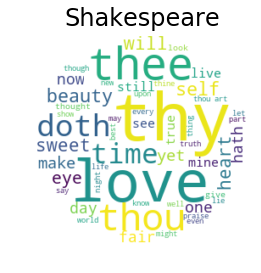
\includegraphics[width=8cm]{Picture/All}
\end{center}
We can see that the top 3 words are thy, love, and thee. \\
Next, we used visualize_sparsities to visualize the sparsities of the A and O matrices. 
\begin{center}
	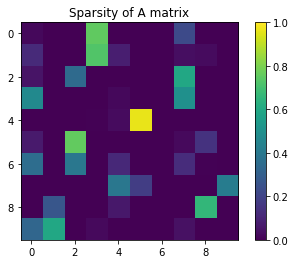
\includegraphics[width=8cm]{Picture/A}
	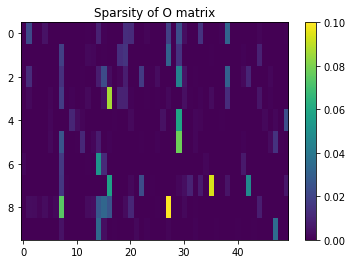
\includegraphics[width=8cm]{Picture/O}
\end{center}
We can see that our A and O matrix and both pretty sparse, our observation matrix in particular is very sparse. This means that observation from a state or to a state is very unlikely. \\
Next, we use states_to_wordclouds to represent each state. We see that for 5 states, the top 10 words in each state are: \\
\begin{verbatim}
State 1: love, thy, ill, see, know, doth, upon, hold, thing, hath
State 2: thou, make, thy, yet, still, every, time, tell, thee, see
State 3: will, hath, doth, now, dost, may, even, whilst, though, never
State 4: thy, thee, thine, mine, one, love, art, wilt, dost, others
State 5: love, eye, self, beauty, thou, sweet, time, heart, day, will
\end{verbatim}
We can see that thy, thee, and love are very common among all 5 states. State 1 seem more general. State 2 seems to contain adverbs. State 3 seems to contain action. State 4 seems to contain pronouns. State 5 seems to contain adjective related to love. \\
Lastly, we used animate_emissions to see how the model transitions between states. In our case, we have 5 states and string of 10 words. We can see that the arrows show the transitions between states. We also see the likelihood of transitions. Arrows with darker colors are more likely while the fainter ones are less likely. 
\begin{center}
	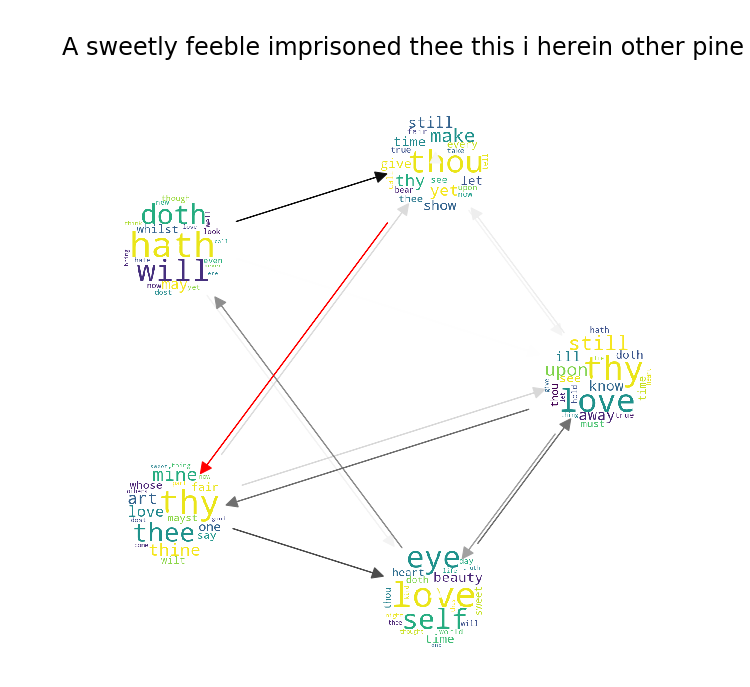
\includegraphics[width=14cm]{Picture/Vis}
\end{center}
% Explain your interpretation of how a Hidden Markov Model learns patterns in Shakespeare's texts. You should briefly elaborate on the methods you used to analyze the model. In addition, for at least 5 hidden states give a list of the top 10 words that associate with this hidden state and state any common features among these groups. Furthermore, try to interpret and visualize the learned transitions between states. A possible suggestion is to draw a transition diagram of your Markov model and give descriptive names to the states. Feel free to be creative with your visualizations, but remember that accurately representing data is still your primary objective. Your figures, tables, and diagrams should contribute to a discussion about your model.

\end{document}
